\documentclass{school}
% using the school template from https://github.com/re1/latex-templates
% \usepackage{minted}
% \usemintedstyle{lovelace}

\subject{Angewandte Mathematik}
\title{Unendliche Folgen und Reihen}
\subtitle{Jahrgang 4 \-- Semester 2 \-- Schularbeit 3}

\author{Markus Reichl}

\begin{document}

\maketitle

\tableofcontents

\newpage

\section{Wiederholung und Vertiefung}
\subsection{Mengen und Folgen}
\begin{tabular}{l l l}
& \textbf{Mengen} & \textbf{Folgen}\\
\midrule
Formel & Mengenklammer \{\} & Folgenklammer <>\\
Enthalten & Elemente & Glieder\\
Aufzählung & $\{1, 2, 3\}$ & $<1, 2, 3>$\\
Beschreibung & $\{n \text{ e } N \text{ | } 0 < n < 4\}$ & $<a_i+1 = a_i + 1>$\\
Inhalt & Reihenfolge ist irrelevant & Reihenfolge ist wesentlich
\end{tabular}

\subsection{Spezielle Folgen}
\begin{tabular}{l l l}
& \textbf{Arithmetische Folgen} & \textbf{Geometrische Folgen}\\
\midrule
Bildungsgesetz & $<a_1, a_2, a_3, \cdots>$ & $<b_1, b_2, b_3, \cdots>$\\
\small{Implizit}& $\rightarrow a_{n+1} = a_n + d$ & $\rightarrow b_{n+1} = b_n * q$\\
\small{Explizit}& $\rightarrow  a_n = a_0 + n * d$ & $\rightarrow b_n = b_0 * q ^ n$\\
& $\rightarrow  a_n = a_1 + (n-1) * d$ & $\rightarrow b_n = b_1 * q^{n - 1}$\\
\midrule
Mittel & $a_n = \frac{a_{n-1} + a_{n+1}}{2}$ & $a_n = \sqrt{a_{n-1} * a_{n+1}}$ \\
\midrule
Summenformel & $s_n = \sum_{i=0}^n a_0 + i * d$ & $s_n=a_0\sum_{i=0}^{n} q^i$\\
& $s_n = (n + 1) * \frac{a_0 + a_n}{2}$ & $s_n = b_0 * \frac{q^{n + 1} - 1}{q - 1}$\\
& $s_n = (n + 1) * (a_0 + \frac{n * d}{2})$ & $s_n = b_1 * \frac{q^n - 1}{q - 1}$\\
& $s_n = n * \frac{a_1 + a_n}{2}$ &\\
& $s_n = n * (a_1 + \frac{(n - 1) * d}{2})$ &\\
\midrule
Spezialfälle & & $q > 1$ Limes gegen unendlich\\
& & $q = 1$ Konstant $\rightarrow$ Limes gegen $b_1$\\
& & $0 < q < 1$ Limes gegen 0
\end{tabular}

\newpage

\section{Wirtschaftsmathematik}
\subsection{Abschreibungen}
Wirtschaftsgüter verlieren mit der Zeit ihren Wert, dementsprechend spricht man von einem \textbf{Buchwert} und einem \textbf{Restwert}.
Die Art der Wertminderung und die Aufteilung auf die Nutzungsdauer nennt sich \textbf{Abschreibung}.
Der Nutzwert eines Objekts ergeben sich aus der folgenden Gleichung, beziehungsweise Reihe:
$${R_1}={R_0}-{A_1}$$
$$\downarrow$$
$${R_n = R_{n-1} - A_n}$$
\vspace{0.5 em}
$$R_{n-1} =\text{ Anschaffungskosten}$$
$$R_{n} =\text{ Restwert nach einem Jahr}$$
$$A_{n} =\text{ Abschreibung}$$

\subsubsection{Lineare Abschreibung}
Bei einer linearen Abschreibung ist der jährliche Abschreibungswert konstant.
$$R_1 = R_0 - A$$
$$\downarrow$$
$$R_n = R_{n-1} - A$$
$$R_n = R_0 - A * n$$
\paragraph{Beispiel:}
$$\text{Preis} = 65 000\text{ Euro}$$
$$\text{Nutzungsdauer} = 5\text{ Jahre}$$
$$\text{Schrottwert} = 5000\text{ Euro}$$
\\
\begin{tabular}{c l l l}
\textbf{Jahr} & \textbf{Restwert zu Jahresbeginn} & \textbf{Abschreibung} & \textbf{Restwert zu Jahresende}\\
\midrule
1 & 65 000 & 12 000 & 53 000\\
2 & 53 000 & 12 000 & \dots \\
3 & \dots & 12 000 & \dots \\
4 & \dots & 12 000 & 5 000\\
\end{tabular}

\newpage
\subsubsection{Geometrisch Degressive Abschreibung}
Bei einer geometrisch degressiven Abschreibung wird jährlich ein Prozentsatz $i$ des Restwertes $R$ abgeschrieben.
$$R_1 = R_0 - R_0 * i$$
$$\downarrow$$
$$R_n = R_{n-1} * (1 - i)$$
$$R_n = R_0 * {(1 - i)}^n$$
\vspace{0.5 em}
$$R =\text{ Restwert}$$
$$i =\text{ Zinsen}$$

\paragraph{Beispiel} ~\\
\begin{tabular}{c l l l}
\textbf{Jahr} & \textbf{Restwert zu Jahresbeginn} & \textbf{Abschreibung} & \textbf{Restwert zu Jahresende}\\
\midrule
0 & 65 000 & 40\% & 39 000\\
1 & \dots & 40\% & \dots \\
2 & 26 000 & 40\% & 23 400\\
3 & \dots & 40\% & \dots \\
\midrule
0 & $R_0$ & $A_0 = R_0 * i$ & $R_1 = R_0 - A_0 = R_0 * (1-i)$\\
1 & $R_1 = R_0 * (1-i)$ & $A_1 = R_1 * i$ & $R_2 = R_1 - A_1 = R_1 * {(1-i)}^2$\\
n & $R_n = R_0 * (1-i)^n$& $A_n = R_n * i$ & $R_{n + 1} = R_{n} - A_{n}$\\
\end{tabular}

\subsection{Rente}
Eine Rente ist eine Folge von Zahlungen, in gleicher Höhe und in gleichen Zeitabschnitten.
Erfolgt die Zahlung zu Beginn des Zeitabschnitts, ist sie \textbf{vorsch\"ussig}, erfolgt sie am Ende ist sie \textbf{nachsch\"ussig}.
Die Anzahl der Zeitabschnitte definiert die \textbf{Laufzeit}.
\vspace{1 em}\\
\textbf{Beispiele: } R\"uckzahlung von Krediten, Versicherungen, Alterspension, \dots

\begin{center}
    \begin{tabular}{l | l l}
    & \textbf{nachsch\"ussig} & \textbf{vorsch\"ussig}\\
    \hline
    \textbf{Endwert} (Aufzinsen) & $E_n = R_0*\frac{q^n - 1}{q - 1}$ & $E_v = R_0*q*\frac{q^n - 1}{q - 1}$\\
    \textbf{Barwert} (Abzinsen) & $B_n = \frac{E_n}{q^n}$ & $B_v = \frac{E_v}{q^n}$
    \end{tabular}
\end{center}
$$R = \text{Restwert}$$
$$q = 1 + i$$
$$i = \text{Zinsen}$$

\newpage
\subsection{Kredittilgung}
Die Kredittilgung beschreibt die Ver\"anderung einer \textbf{Schuld} zu einem bestimmten \textbf{Zinssatz}, über eine vorgegebene \textbf{Laufzeit}, um einen fixierten Betrag, die \textbf{Annuität}.
\\Die Differenz zwischen alter und neuer Schuld nennt sich \textbf{Tilgung}.
\paragraph{Annuität}~\\
Die Annuität $A$ wird auch Wiedergewinnungswert oder Anniutätenfaktor genannt und ist als Kehrwert des Barwerts $B$ definiert.

\paragraph{Nachschüssig}
$$A_N=R_0 * q^n * \frac{q-1}{q^n-1}$$
\vspace{0.5 em}
$$Z_n=R_n * i$$
$$T_n=Z_n - A$$
$$R_{n+1} = R_n - T_n$$
$$\downarrow$$
$$R_{n} = R_{n-1} * q - A$$
$$R_n = R_0 * q^n - \sum^{n-1}_{i = 0}{A * q^i}$$
\paragraph{Vorschüssig}
$$A_V=R_0 * q^{n-1} * \frac{q-1}{q^n-1}$$
\vspace{0.5 em}
$$T_n=(R_n - A) * i$$
$$R_{n+1} = R_n - T_n$$
$$\downarrow$$
$$R_{n} = (R_{n-1} - A) * q$$
$$R_n = R_0 * q^n - \sum^{n}_{i = 1}{A * q^i}$$
\vspace{0.5 em}
$$A = \text{Annuität},~ R = \text{Restschuld},~ n = \text{Laufzeit},~ q = 1 + i,~ i = \text{Zinssatz}$$
$$Z = \text{Zinsen},~ T = \text{Tilgung}$$

\subsubsection{Tilgungsplan}
Ein Kredit von 10 000 Euro, \"uber 4 Jahre, zu einem Zinssatz von 10\% wird zur\"uckgezahlt. Dieser Prozess soll anhand einer Tabelle dargestellt. Die Rentenzahlung erfolgt zu Jahresende.
\vskip 2 mm
\begin{tabular}{c l l l l l}
\textbf{Jahr} & \textbf{Schuld} & \textbf{Zinsen} & \textbf{Annuität} & \textbf{Tilgung} & \textbf{Restschuld}\\
\hline
1 & 10000 & 1000 & 3154.71 & 2154.71 & 7845.29\\
2 & 7845.29 & 784.53 & 3154.71 & 2370.18 & 5475.11\\
3 & 5475.11 & 547.51 & 3154.71 & 2607.20 & 2867.92\\
4 & 2867.92 & 286.79 & 3154.71 & 2867.92 & 0 $\rightarrow$ Schuld beglichen!
\end{tabular}

\subsection{Angebotsrechnung}
Die Angebotsrechnung vergleicht verschiedene Angebote auf ihren langfristigen Nutzen.
Die Berechnung ähnelt dabei der Kredittilgung, nur wird hier die Annuität addiert.
\paragraph{Nachschüssig}
$$K_n = K_{n-1}*q + A$$
$$K_n = K_0 * q^n + \sum^{n-1}_{i = 0}{A * q^i}$$
\paragraph{Vorschüssig}
$$K_n = (K_{n-1} + A) * q$$
$$K_n = K_0 * q^n + \sum^{n}_{i = 1}{A * q^i}$$
\vspace{0.5 em}
$$K = \text{Kapital},~ A = \text{Annuität},~ q = 1 + i,~ i = \text{Zinssatz}$$

\paragraph{Äquivalenzprinzip}~\\
Zahlungen dürfen nur verglichen werden, wenn diese am selben Stichtag verzinst wurden.

\paragraph{Beispiel} ~\\
Gegeben sei eine Firma, mit 2 Angeboten zu einem Kalkulationszinssatz von 5\% pro Jahr:\\
$~\to \quad$\textbf{Angebot A:} 8 Millionen Euro sofort und dann 7 mal 2 Millionen Euro zu Jahresende\\
$~\to \quad$\textbf{Angebot B:} 5 mal 4 Millionen Euro zu Jahresende
\vspace{1 em}\\
\textbf{Vergleich:}
\begin{center}
    \begin{tabular}{l | l l l l l l l l l}
    & 0 & 1 & 2 & 3 & 4 & 5 & 6 & 7 & Jahre\\
    \hline
    A & 8 & 10.4 & 12.92 & 15.57 & 18.34 & 21.26 & 24.32 & 27.54 & Mio. Euro\\
    \hline
    B & 0 & 4 & 8.2 & 12.61 & 17.24 & 22.10 & & &
    \end{tabular}
\end{center}
\vskip 2 mm ~\\
Das Angebot A ist für den Abnehmer besser geeignet, da dieses auf Dauer mehr einbringt.

\section{Potenzreihen}
\subsection{Einführung}
\subsubsection{Definition}
\begin{flushleft}
Ist $<a_n>$ eine Folge von Zahlen und $x_0 \in \mathbb{C}$ dann ist die Reihe $\sum_{n=0}^\infty a_n*x^n$ eine \textbf{Potenzreihe} mit dem \textbf{Entwicklungspunkt} $x_0$.
\end{flushleft}
Die Potenzreihe ist also die Summe einer Reihe $<a_n * x^n = a_0 + a_1 * x^1 + a_2 * x^2 + ... + a_n * x^n>$, wobei $a_n$ den Koeffizienten des Glieds $x^n$ darstellt.

\subsubsection{Konvergenzradius}
Der Konvergenzradius $R$ einer Potenzreihe, ist als das Supremum aller Zahlen $\geq 0$ definiert, für welche mindestens ein x mit $|x| < R$ konvergiert\footnote{Besitzt eine Folge einen Grenzwert, wird sie konvergent, andernfalls divergent genannt.}.
\vspace{1 em}\\
Wenn $a_{n} \neq 0$ gilt und der angegebene Limes existiert, dann kann der Konvergenzradius wie folgt berechnet werden.
$$R = \lim\limits_{n \to \infty} |\frac{a_n}{a_{n+1}}|$$

\subsubsection{Idee}
Anstatt eine Funktion $f(x)$ auszuwerten, entwickelt man eine Potenzreihe\\
$\to$ Es werden Zahlenwerte für die einzelnen Koeffizienten berechnet.
\paragraph{Beispiel:} $$sin(x) = x - \frac{x^3}{6} + \frac{x^5}{120} - \frac{x^7}{5040} \pm ... \pm \frac{x^n}{n!}$$

\subsubsection{Verwendung}
\begin{itemize}
 \item Berechnung von Funktionswerten
 \item N\"aherungsformeln
 \item Integration
\end{itemize}

\newpage
\subsection{Anwendung}
Angenommen man w\"usste die Entwicklung einer Potenzreihe $f(x)$ als $$f(x) = a_0 + a_1*x + a_2*x^2 + ... + a_n*x^n$$ und nehme an, die Zahlen wären bestimmt. Dann könne man anschreiben:
\[f(x)=a_3*x^3+a_2*x^2+a_1*x+a_0\]
\[f'(x)=3*a_3*x^2+2*a_2*x+a_1\]
\[f''(x)=5*a_3*x+2*a_2\]
\[f'''(x)=6*a_3\]
Wobei gilt:
$$f(0)=a_0$$
$$f'(0)=a_1$$
$$\frac{1}{2}*f''(0)=a_2$$
$$\frac{1}{6}*f'''(0)=a_3$$
\\
Der Wert von $f(0)$ ist bei vielen Funktionen bekannt (z. B.: $sin(0) = 0$, $cos(0) = 1$) und der Quotient ergibt sich aus der Fakultät\footnote{Produkt aller Zahlen von $1$ bis $n$\\Bsp.: $3! \to 1 * 2 * 3 = 6$} $(!)$ des Grades der Ableitung $^(n)$.
\vskip 0.5 mm ~\\
Daraus ergibt sich folgende Regel f\"ur die Stelle $f(0)$:
\[f(0)=\sum_{n=0}^{\infty }{\left. \frac{{{f}^{(n)}(0)}\, {{x}^{n}}}{n!}\right.}\]

\newpage
\subsection{Taylorreihe}
Eine Funktion, die unendlich oft differenzierbar ist, bildet eine Taylorreihe. Diese dient zur N\"aherung an eine Funktion, an einer bestimmten Stelle.
\footnote{Taschenrechner beispielsweise nutzen Taylorreihen, um den Sinus und andere trigonometrische Funktionen zu berechnen, was sonst zu rechenintensiv wäre.}
\vskip 0.5 mm ~\\
Die hergeleitete Funktion stellt eine spezielle Form der Taylorreihe mit der Entwicklungsstelle $a = 0$ dar. Diese Reihe wird auch \textbf{MacLaurin-Reihe} genannt.

\subsubsection{Definition}
Eine Funktion $f(x)$ entspricht einer \textbf{Taylorreihe} mit unendlich vielen \textbf{Gliedern}. Die Stelle $a$ ist die \textbf{Entwicklungsstelle}, in deren Umgebung die Funktion beobachtet wird.
$$f(x)=\sum_{n=0}^\infty \frac{f^{(n)}(a)}{n!}*(x-a)^n$$
Jedes Glied einer Taylorreihe entspricht mit seinen Vorgängern einem Taylorpolynom\footnote{Eine Taylorreihe mit n Gliedern nennt man auch eine Taylorreihe n-ten Grades.}. Je mehr Polynome (je höher der Grad), desto genauer ist die Näherung.

\paragraph{Beispiel}
Eine einfache Taylorreihe bildet die N\"aherung an den Sinus. Daf\"ur sind zun\"achst einmal die Ableitungen wichtig, welche sind:
$$f(x) = sin(x)$$
$$f'(x) = cos(x)$$
$$f''(x) = -sin(x)$$
$$f'''(x) = -cos(x)$$
$$f''''(x) = sin(x)$$
Wie man sieht ist die Ableitung beliebig oft wiederholbar und nach 4 durchg\"angen wieder beim Ursprung. Dieses Wissen in die Taylorreihe eingesetzt f\"uhrt zu folgender Reihe.
$$sin(x)=\sum_{n=0}^\infty \frac{sin(a)^{(n)}}{n!}*(x-a)^n$$
\newpage~\\
In diesem Fall ist die Umgebung $0$ interessant, also wird dieser Wert eingesetzt, was zu einer MacLaurin-Reihe f\"uhrt.
$$sin(x)=\sum_{n=0}^\infty \frac{sin(0)^{(n)}}{n!}*x^n$$
Damit kann der Sinus auf einen beliebigen Genauigkeitsgrad bestimmt werden.\\
Als Beispiel werden hier 5 Glieder berechnet.
$$sin(x)=\frac{sin(0)}{0!}*x^0 + \frac{sin(0)'}{1!}*x^1 + \frac{sin(0)''}{2!}*x^2 + \frac{sin(0)'''}{3!}*x^3 + \frac{sin(0)''''}{4!}*x^4$$
$$\downarrow$$
$$sin(x)=sin(0) + \frac{cos(0)}{1!}*x - \frac{sin(0)}{2!}*x^2 - \frac{cos(0)}{3!}*x^3 + \frac{sin(0)}{4!}*x^4$$
$$\downarrow$$
$$sin(x)=\frac{x}{1} - \frac{x^3}{3!} + \frac{x^5}{5!} \pm ...$$
\\
Diese Formel resultiert bereits in ein relativ genaues Ergebnis.

\paragraph{Grafisch} ~\\ Grafisch kann dieser Prozess wie folgt veranschaulicht werden:
\begin{figure}[hh]
\centering
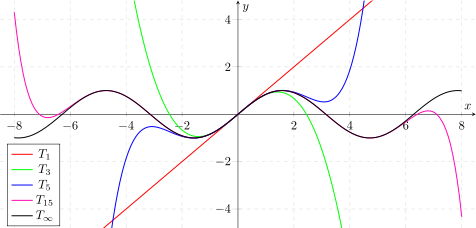
\includegraphics[width=0.6\textwidth]{sinx-taylor.png}\\
\caption[https://de.wikipedia.org/wiki/Datei:Taylorpolynom-sin.svg]{Taylorreihe sin(x)}
\end{figure}

\newpage

\subsubsection{Euler'sche Formel}
Ein weiteres Beispiel f\"ur die Anwendung von Taylorreihen ist die Euler'sche Formel, welche zur Darstellung von komplexen Zahlen verwendet wird.
$$e^{j*\varphi}=cos(\varphi)+j*sin(\varphi)$$
$$j = \sqrt{-1}, \varphi = \text{Realteil}$$
Eine Exponentialfunktion l\"asst sich anhand einer Taylorreihe darstellen. Unter Verwendung der Funktion ergibt sich dabei folgende Reihe.
$$e^x=\sum_{n=0}^\infty \frac{{e^{0}}^{(n)}}{n!}*x^n$$
Es gilt dabei $e^0 = 1$ und ${e^x}^\text{'} = e^x$, die Funktion kann also vereinfacht werden.
$$e^{j*\varphi}=\sum_{n=0}^\infty \frac{1}{n!}*j*\varphi$$
Als Taylorreihe 4. Grades:
$$e^{j*\varphi}=1 + j*\varphi + \frac{j*\varphi}{2!} + \frac{j*\varphi}{3!} + \frac{j*\varphi}{4!} \pm ...$$
Durch aufl\"osen von $j$:
$$e^{j*\varphi}=1 - \frac{\varphi^2}{2!} + \frac{\varphi^4}{4!} \pm ... + j * (\varphi - \frac{\varphi^3}{3!} + \frac{\varphi^5}{5!} \pm ...)$$
Es handelt sich hierbei offensichtlich um die Taylorreihen des Cosinus und des Sinus. Man könnte also auch einfach schreiben:
$$e^{j*\varphi}=cos(\varphi)+j*sin(\varphi)$$

\newpage

\subsection{N\"aherungsformeln}
\subsubsection{Multiplikation}
Die Multiplikation nach der Reihenentwicklung erlaubt das Multiplizieren zweier Teil-Reihen.

\paragraph{Beispiel}
$$e^{-\frac{x}{3}}*sin(2*x)$$
Wird gen\"ahert berechnet durch:
$$taylor(e^{-\frac{x}{3}})*taylor(sin(2*x))$$
$$\downarrow$$
\[2 x+\mbox{...} * 1-\frac{x}{3}+\frac{{{x}^{2}}}{18}+\mbox{...}\]
$$\downarrow$$
\[2 x-\frac{2 {{x}^{2}}}{3}+\mbox{...}\]

\subsubsection{Integration}
Viele Funktionen sind an sich nicht l\"osbar und m\"ussen daher gen\"ahert werden.
Da eine gesamte Taylorreihe gliedweise integriert werden kann, eignet sich diese perfekt.

\paragraph{Beispiel}
$$G(u) = 0.5 * \frac{1}{\sqrt{2*\pi}}*\int_0^1 e^{- \frac{x^2}{2}}$$
Diese Funktion ist aufgrund ihres Integrals nicht berechenbar und soll daher als Taylorreihe dargestellt werden.
Da diese integriert werden kann wird einfach eingesetzt:
$$G(u) = 0.5 * \frac{1}{\sqrt{2*\pi}}*\int_0^1 taylor(e^{- \frac{x^2}{2}})$$
$$\downarrow$$
$$G(u) = 0.5 * \frac{1}{\sqrt{2*\pi}}*\int_0^1 1-\frac{{{x}^{2}}}{2}+\frac{{{x}^{4}}}{8}-\frac{{{x}^{6}}}{48}+\frac{{{x}^{8}}}{384}-\frac{{{x}^{10}}}{3840}+\mbox{...}$$
$$\downarrow$$
\[G(u) = 0.5-\frac{63 {{u}^{11}}-770 {{u}^{9}}+7920 {{u}^{7}}-66528 {{u}^{5}}+443520 {{u}^{3}}-2661120 u}{10395 {{2}^{\frac{17}{2}}}\, \sqrt{\ensuremath{\pi} }}\]
$$\downarrow$$
$$G(u) = 0.8413441191604388$$

\newpage

\subsubsection{Grenzwerte}
\"Ahnlich wie bei der Integration k\"onnen auch manche Grenzwerte nicht berechnet werden.
Diese k\"onnen ebenso mit der Taylorreihe gen\"ahert werden, da auch der Grenzwert einer Reihe bestimmt werden kann.

\paragraph{Beispiel}
\[\lim_{x\to0}{\frac{\operatorname{xsin}(x)}{x}}\]
Dieser Grenzwert kann nicht berechnet werden da 0 durch 0 dividiert werden w\"urde. Stattdessen kann man jedoch schreiben:
$$\lim_{x\to0} 1-\frac{{{x}^{2}}}{6}+\frac{{{x}^{4}}}{120}-\frac{{{x}^{6}}}{5040}+\frac{{{x}^{8}}}{362880}-\frac{{{x}^{10}}}{39916800}+\text{...}$$
$$\downarrow$$
$$1$$

\printglossaries

\begin{thebibliography}{1}

\bibitem{mathguru-taylorreihe} http://matheguru.com/analysis/88-taylorreihe.html

\bibitem{tugraz-potenzreihen} https://www.math.tugraz.at/~ganster/lv\_differenzialrechnung/06\_potenzreihen.pdf

\bibitem{bislins-eulerformel} http://walter.bislins.ch/blog/index.asp?page=Eulerformel

\bibitem{wikipedia-annuität} https://de.wikipedia.org/wiki/Annuitätendarlehen

\bibitem{wikipedia-tilgungsplan} https://de.wikipedia.org/wiki/Tilgungsplan

\bibitem{lernhelfer-arithmetisch} https://www.lernhelfer.de/schuelerlexikon/mathematik/artikel/arithmetische-folgen

\bibitem{wikipedia-grenzwert} https://de.wikipedia.org/wiki/Grenzwert\_(Folge)

\end{thebibliography}

\listoffigures

\end{document}
